\section{问题描述}

稀疏矩阵 (sparse matrix), 在数值分析中, 是其元素大部分为零的矩阵. 反之, 如果大部分元素都非零, 则这个矩阵是稠密 (dense) 的. 在科学与工程领域中求解线性模型时经常出现大型的稀疏矩阵.

在使用计算机存储和操作稀疏矩阵时, 经常需要修改标准算法以利用矩阵的稀疏结构. 由于其自身的稀疏特性, 通过压缩可以大大节省稀疏矩阵的内存代价. 更为重要的是, 由于过大的尺寸, 标准的算法经常无法操作这些稀疏矩阵.

式 \ref{eq_1_smat_example} 描述了一个 $5 \times 5$ 的稀疏矩阵, 其中只有四个元素为非零值. 为了清楚起见, 零用点表示.
\begin{equation}
    \begin{bmatrix}
        \cdot & 1 & \cdot & \cdot & \cdot \\
        \cdot & \cdot & \cdot & \cdot & \cdot \\
        \cdot & \cdot & \cdot & 2 & \cdot \\
        \cdot & 3 & \cdot & \cdot & \cdot \\
        \cdot & \cdot & \cdot & 4 & \cdot \\
    \end{bmatrix}
    \label{eq_1_smat_example}
\end{equation}

稀疏矩阵的存储可以使用十字链表等方式储存. 可以将矩阵中的非零元表示为链表中的节点, 指向其同行和同列之后的节点, 就组成了十字链表, 便于元素的访问和增删等操作. 每个链表节点除了储存自身的行列位置信息和值外, 还储存了同行列下一个非零节点的指针信息, 构成了二维形式的链表.

在本次实践作业中, 需要基于十字链表实现对稀疏矩阵的创建, 储存和加法, 减法, 乘法, 转置等运算操作, 也可以自行添加新的数据导入导出, 矩阵运算等操作. 其中至少需要实现稀疏矩阵的创建和输入输出, 加法, 减法, 乘法和转置操作, 并给出相应算法的复杂度分析. 对于运算操作中可能出现的错误如尺寸不匹配, 不可逆 (若实现了求逆操作) 等情况, 需要能够捕获错误并提示. 在代码实现过程中还需要避免可能发生的内存泄漏.

本报告中附有针对 2023-2024 学年第一学期 “程序设计与算法基础” 课程的思政报告, 见附录 \ref{appendix_ideology}.

\section{主要算法}

\subsection{数据结构描述}

一个完整的十字链表可以表示为四元组 $M = \langle \bm{s} \in \mathbb{Z}_{+}^{2}, \bm{r}, \bm{c} \rangle,$ 其中各分量分别表示形状、 行首数组、 列首数组和数据节点集合. 对于矩阵中的所有非零元, 存在 $n = \left\langle v, \bm{a} \right\rangle,$ 其中 $\bm{a}$ 为各维度上的坐标与邻接信息数组, 每个 $\bm{a}$ 的分量都可以表示为三元组 $\bm{a}[j] = \left\langle i \in \mathbb{Z}_+, prev, next\right\rangle,$ 分别为该元素在该维度中的下标、 前驱和后继. 对于每个存在非零元的行或列, 其行、 列首数组的相应位置存在指向该行或列的首个非零元素的一条边. 所有分量均由 0 开始标号.

在本文中, 当遇到不指向任何有意义节点的边时, 我们使用 $\Lambda$ 表示该边. 实际上, 在算法实现中, 我们使用特殊指针值 \texttt{NULL} 实现 $\Lambda.$

\newcommand{\Prec}[2]{\mathsf{Prec}(#1, #2)}
\newcommand{\Succ}[2]{\mathsf{Succ}(#1, #2)}
\newcommand{\Index}[2]{\mathsf{Index}(#1, #2)}
为方便讨论, 我们引入表示十字链表中节点 $n$ 在 $d$ 维方向的前驱、 后继与下标的记号:
\begin{equation}
    \begin{aligned}
        \Prec{n}{d} & = n.\bm{a}[d].prev\\
        \Succ{n}{d} & = n.\bm{a}[d].next\\
        \Index{n}{d} & = n.\bm{a}[d].i\\
    \end{aligned}
\end{equation}

\newcommand{\Elems}[2]{\mathsf{Elems}(#1, #2)}
对于十字链表中的每一维度 $d,$ 我们定义记号 $\Elems{\cdot}{\cdot}$ 表示该链表上的所有元素集合:
\begin{equation}
    \Elems{n}{d} = \begin{cases}
        \emptyset & \text{if}\ n = \Lambda,\\
        \left\{n\right\} \cup \Elems{\Succ{n}{d}}{d} & \text{otherwise}.\\
    \end{cases}
\end{equation}

\newcommand{\Nodes}[1]{\mathsf{Nodes}(#1)}
基于上述定义, 我们不难定义记号 $\Nodes{\cdot}$ 表示稀疏矩阵中的所有链表节点的集合:
\begin{equation}
    \Nodes{M} = \bigcup_{h \in M.\bm{r}} \Elems{h}{1}.
\end{equation}

\subsection{矩阵建立与销毁}

算法 \ref{algo_smat_new} 给出了创建一个具有给定形状 $\bm{s} \in \mathbb{R}^2$ 且元素全为 0 的系数矩阵的过程. 不难发现, 基于十字链表的稀疏矩阵在创建时并不需要为任何元素分配实际的存储空间. 实际实现中, 创建时的内存开销主要集中于为 $\bm{r}$ 和 $\bm{c}$ 所分配的空间上. 若不考虑空间分配的时间, 该算法可以在 $\mathcal{O}(1)$ 时间内完成.
\begin{breakablealgorithm}
\caption{创建稀疏矩阵.}
\label{algo_smat_new}
\begin{algorithmic}[1]
\Require 矩阵形状 $\bm{s} \in \mathbb{R}^2.$
\Ensure 指定形状的全零矩阵.
\Function{SMatrix-New}{$\bm{s}$}
    \State $\bm{r} \gets$ 长度为 $\bm{s}[0]$ 的数组, 元素全为 $\Lambda$
    \State $\bm{c} \gets$ 长度为 $\bm{s}[1]$ 的数组, 元素全为 $\Lambda$
    \State \Return $\left\langle \bm{s}, \bm{r}, \bm{c} \right\rangle$
\EndFunction
\end{algorithmic}
\end{breakablealgorithm}

算法 \ref{algo_smat_free} 给出了释放一个稀疏矩阵的过程. 在二维稀疏矩阵中, 显然, 我们只需要对沿其中一个维度进行元素释放, 便可以完全释放所有数据节点. 该算法需要遍历所有非零节点, 依次对其进行释放操作. 设矩阵中共有 $n$ 个非零元素, 那么该算法需要 $\mathcal{O}(n)$ 的运行时间.
\begin{breakablealgorithm}
\caption{释放稀疏矩阵.}
\label{algo_smat_free}
\begin{algorithmic}[1]
\Require 稀疏矩阵 $M$.
\Procedure{SMatrix-Free}{$M$}
    \For{$h \in \{ r \mid r \in M.\bm{r} \land r \neq \Lambda \}$}
        \State $p \gets r$
        \While{$p \neq \Lambda$}
            \State $t \gets \Succ{p}{1}$
            \State 释放 $p$ 的空间
            \State $p \gets t$
        \EndWhile
    \EndFor
    \State $M.\bm{s} \gets (0, 0)$
    \State 释放 $M$ 及其所有分量的空间
\EndProcedure
\end{algorithmic}
\end{breakablealgorithm}

\subsection{矩阵元素访问}

算法 \ref{algo_smat_rand_at} 描述了稀疏矩阵的下标 (随机访问) 操作. 该算法中, 对给定坐标的第一次寻址为偏移操作, 仅需要常数时间即可完成; 对给定坐标的第二次寻址为链表查找操作, 最坏情况下则需要遍历整个链表. 假如我们将每行中的非零元数量记为 $n,$ 那么其最坏情况下与平均情况下都需要 $\mathcal{O}(n)$ 的时间进行查找.
\begin{breakablealgorithm}
\caption{稀疏矩阵的随机访问.}
\label{algo_smat_rand_at}
\begin{algorithmic}[1]
\Require 稀疏矩阵 $M,$ 待查坐标 $P \in \mathbb{Z}_{+}^{2}.$
\Ensure 位于该坐标处的元素 $n$ 与其值 $v.$
\Function{SMatrix-Random-At}{$M, P$}
    \State $p \gets M.\bm{r}[P[0]]$
    \While{$p \neq \Lambda$}
        \If{$P[1] = \Index{p}{1}$}
            \State \Return $\left\langle n=p; v=p.v \right\rangle$
        \EndIf
        \State $p \gets \Succ{p}{1}$
    \EndWhile
    \State \Return $\left\langle n=\Lambda; v=0 \right\rangle$
\EndFunction
\end{algorithmic}
\end{breakablealgorithm}

\paragraph{特定于顺序访问的优化} 很多情况下, 对矩阵元素的查找具有空间局部性, 即所查找下标中仅有少数几个维度分量变化较快. 假如我们使用 \textsc{SMatrix-Random-At} 在二维稀疏矩阵中对一整列或一整行进行顺序访问, 我们将观察到相当不理想的性能表现, 因为在该过程中需要进行 $(n^2 + n) / 2$ 次后继操作, 并没有充分利用有序访问的局部性特征. 算法 \ref{algo_smat_cont_at} 仅适用于有序的查找需求, 且对调用方式有更严格的规定, 但是它与算法 \ref{algo_smat_rand_at} 相比有显著的性能优势: 仅需要调用 $n$ 次即可搜索整个指定维度.
\begin{breakablealgorithm}
\caption{稀疏矩阵的迭代式顺序访问.}
\label{algo_smat_cont_at}
\begin{algorithmic}[1]
\Require 当前矩阵数据元素 $n,$ 待搜索的下标 $i,$ 待搜索的维度序号 $d.$
\Ensure 该坐标处的元素值 $v,$ 更新后的当前元素 $n'.$
\Function{SMatrix-Continuous-At}{$n, i, d$}
    \If{$n = \Lambda$}
        \State \Return $v=0; n'=\Lambda$
    \EndIf
    \State $p \gets \Succ{n}{d}$
    \If{$\Index{n}{d} = i$}
        \State \Return $\left\langle v=n.v; n'=p \right\rangle$
    \EndIf
    \State \Return $\left\langle v=0; n'=n \right\rangle$
\EndFunction
\end{algorithmic}
\end{breakablealgorithm}

\subsection{矩阵元素修改}

\paragraph{元素置零} 将稀疏矩阵中的元素置为 $0$ 等价于将其从链表中删除. 算法 \ref{algo_smat_remove_along} 是执行删除操作的步骤, 它描述了将待删除节点从某一特定维度上移除的操作, 该算法能在常数时间内执行完毕. 算法 \ref{algo_smat_remove} 则由一次查找和两次移除组成, 它执行包括释放节点占用空间在内的完整删除操作. 它的运行时间由查找的运行时间决定. 
\begin{breakablealgorithm}
\caption{沿稀疏矩阵的某一维度移除元素.}
\label{algo_smat_remove_along}
\begin{algorithmic}[1]
\Require 稀疏矩阵 $M,$ 待删除节点 $n,$ 删除维度 $d.$
\Ensure 节点所在维首的更新值.
\Function{SMatrix-Remove-Along}{$M, n, d$}
    \State $n \gets$ 
    \State $prec \gets \Prec{n}{d}$
    \State $succ \gets \Succ{n}{d}$
    \If{$succ \neq \Lambda$}
        \State $\Prec{succ}{d} \gets prec$
        \State $\Succ{n}{d} \gets \Lambda$
    \EndIf
    \If{$prec \neq \Lambda$}
        \State $\Succ{prec}{d} \gets succ$
        \State $\Prec{n}{d} \gets \Lambda$
    \Else
        \State \Return $succ$
    \EndIf
    \State \Return 不需要更新节点所在维首
\EndFunction
\end{algorithmic}
\end{breakablealgorithm}

\begin{breakablealgorithm}
\caption{移除稀疏矩阵元素.}
\label{algo_smat_remove}
\begin{algorithmic}[1]
\Require 稀疏矩阵 $M,$ 待删除节点坐标 $P.$
\Procedure{SMatrix-Remove}{$M, P$}
    \State $\left\langle n, *\right\rangle \gets \textsc{SMatrix-Random-At}(M, P)$
    \State $\textsc{SMatrix-Remove-Along}(M, n, 0)$
    \State $\textsc{SMatrix-Remove-Along}(M, n, 1)$
    \State $M.N \gets M.N \setminus \{n\}$
    \State 释放 $n$ 的空间
\EndProcedure
\end{algorithmic}
\end{breakablealgorithm}

\paragraph{元素赋非零值} 将稀疏矩阵中的零元设为非零值等价于向链表中插入新的节点, 而将非零元素赋值为另一个非零值则仅仅需要覆写原有节点中的卫星数据. 我们分两部分描述元素插入算法: 算法 \ref{algo_smat_set_along} 沿指定维度插入非零节点, 算法 \ref{algo_smat_set} 执行完整的插入操作. 算法 \ref{algo_smat_set_along} 在最坏情况下需要遍历整个链表才能找到合适的插入位置. 假定插入维度上存在 $n$ 个非零元, 那么它的运行时间为 $\mathcal{O}(n).$ 当该算法发现指定位置已有节点时, 它只是简单的将该已有节点的 $v$ 设为待插入节点的 $v,$ 以避免修改各条边与释放原有节点的时间开销.
\begin{breakablealgorithm}
\caption{沿稀疏矩阵的某一维度修改元素.}
\label{algo_smat_set_along}
\begin{algorithmic}[1]
\Require 稀疏矩阵 $M,$ 待插入节点 $n,$ 节点所在维首 $h,$ 插入维度 $d.$
\Ensure 目标坐标是否已有节点存在.
\Function{SMatrix-Set-Along}{$M, n, h, d$}
    \If{$h = \Lambda$}
        \State $h \gets n$
        \State $\Prec{n}{d} \gets \Lambda$
        \State $\Succ{n}{d} \gets \Lambda$
        \State \Return \textbf{false}
    \EndIf
    \If{$\exists p \in \Elems{h}{d} \mid \Index{p}{d} = \Index{n}{d}$}
        \State $p.v \gets n.v$
        \State \Return \textbf{true}
    \EndIf
    \State 插入 $n$ 使其满足 $\Index{\Prec{n}{d}}{d} < \Index{n}{d} < \Index{\Succ{n}{d}}{d}$
    \State \Return \textbf{false}
\EndFunction
\end{algorithmic}
\end{breakablealgorithm}

算法 \ref{algo_smat_set} 判断待修改的目标值是否为零元, 并据此或在两个维度上依次调用算法 \ref{algo_smat_set_along}, 或调用算法 \ref{algo_smat_remove} 删除零元.
\begin{breakablealgorithm}
\caption{修改稀疏矩阵中的元素.}
\label{algo_smat_set}
\begin{algorithmic}[1]
\Require 稀疏矩阵 $M,$ 待插入坐标 $P \in \mathbb{Z}_{+}^{2},$ 待插入值 $v.$
\Procedure{SMatrix-Set}{$M, P, v$}
    \If{$v = 0$}
        \State $\textsc{SMatrix-Remove}(M, P)$
        \State \Return
    \EndIf
    \State $h_r \gets M.\bm{r}[P[0]]$
    \State $h_c \gets M.\bm{c}[P[1]]$
    \State $n \gets$ 新分配的空节点
    \State $\Index{n}{0} \gets P[0]$
    \State $\Index{n}{1} \gets P[1]$
    \State $d \gets \textsc{SMatrix-Insert-Along}(M, n, h_r, 1) \lor \textsc{SMatrix-Insert-Along}(M, n, h_c, 0)$
    \If{$d$}
        \State 释放 $n$
    \EndIf
\EndProcedure
\end{algorithmic}
\end{breakablealgorithm}

\subsection{基础矩阵算术}

在定义了算法 \ref{algo_smat_rand_at} 描述的随机访问操作后, 矩阵算术可以用 \textit{朴素} (na\"{i}ve) 的逐元素计算法设计. 对于一个 $m \times n$ 的矩阵而言, 朴素加法、 减法、 转置算法需要计算 $mn$ 个值, 并且进行相同数量的插入操作; 对于两个分别为 $m \times k$ 和 $k \times n$ 的矩阵而言, 朴素矩阵乘法需要计算 $mnk$ 个值, 进行 $mn$ 次插入操作. 显然, 这不是很高效的算法, 尤其是在插入操作本身也需要消耗非常数时间的情况下. 幸运的是, 稀疏矩阵的结构允许我们跳过大部分元素的计算, 从而将计算数量降低至与非零元个数相关, 而不是与矩阵形状相关. 在本节中, 提及元素个数或者矩阵形状时, 带撇号的符号一般代表非零元的个数, 不带撇号的符号一般代表矩阵形状的效果值.

\subsubsection{加法与减法}

由于十字链表的元素在所有维度上均是有序的, 我们可以同时对两个操作数矩阵的目标链表进行遍历. 算法 \ref{algo_smat_add_sub} 实现了矩阵上的运算 $C_{ij} = A_{ij} \circ B_{ij},$ 其中 $\circ$ 是任意标量二元操作. 该算法需要执行插入的次数等于集合 $A, B$ 中不同位置非零元的总数, 远小于朴素算法中的形状分量之积.
\begin{breakablealgorithm}
\caption{稀疏矩阵的加法与减法运算.}
\label{algo_smat_add_sub}
\begin{algorithmic}[1]
\Require 稀疏矩阵 $A, B,$ 标量二元操作 $\circ.$
\Ensure 逐元素施加操作 $\circ$ 后的结果矩阵.
\Function{SMatrix-Insert}{$A, B, \circ$}
    \If{$A.\bm{s} \neq B.\bm{s}$}
        \State \textbf{error} 参数矩阵形状不符
    \EndIf
    \State $C \gets \textsc{SMatrix-New}(A.\bm{s})$
    \For{$i \gets 0 \hdots A.\bm{s}[0]$}
        \State $p_A \gets A.\bm{c}[i]$
        \State $p_B \gets B.\bm{c}[i]$
        \While{$p_A \neq \Lambda \lor p_B \neq \Lambda$}
            \If{$p_A \neq \Lambda \land p_B \neq \Lambda$}
                \State $j_A \gets \Index{p_A}{1}$
                \State $j_B \gets \Index{p_B}{1}$
                \If{$j_A < j_B$}
                    \State $\textsc{SMatrix-Set}(C, (i, j_A), p_A.v \circ 0)$
                    \State $p_A \gets \Succ{p_A}{1}$
                \ElsIf{$j_A > j_B$}
                    \State $\textsc{SMatrix-Set}(C, (i, j_B), 0 \circ p_B.v)$
                    \State $p_B \gets \Succ{p_B}{1}$
                \Else
                    \State $\textsc{SMatrix-Set}(C, (i, j_A), p_A.v \circ p_B.v)$
                    \State $p_A \gets \Succ{p_A}{1}$
                    \State $p_B \gets \Succ{p_B}{1}$
                \EndIf
            \ElsIf{$p_A = \Lambda$}
                \State $\textsc{SMatrix-Set}(C, (i, \Index{p_B}{1}), 0 \circ p_B.v)$
                \State $p_B \gets \Succ{p_B}{1}$
            \Else
                \State $\textsc{SMatrix-Set}(C, (i, \Index{p_A}{1}), p_A.v \circ 0)$
                \State $p_A \gets \Succ{p_A}{1}$
            \EndIf
        \EndWhile
    \EndFor
    \State \Return $C$
\EndFunction
\end{algorithmic}
\end{breakablealgorithm}

\subsubsection{乘法}

稀疏矩阵乘法的优化与加减法类似, 如算法 \ref{algo_smat_mul} 所示. 设矩阵 $A$ 中有 $m'$ 个包含非零元素的行, $B$ 中有 $n'$ 个包含非零元素的列, 那么该算法需要执行 $m' n'$ 次插入操作; 计算每个插入的值均需要 $\min\{A\ \text{中该行非零元素数量}, B\ \text{中该列非零元素数量}\}$ 次浮点乘法和加法.
\begin{breakablealgorithm}
\caption{稀疏矩阵的乘法.}
\label{algo_smat_mul}
\begin{algorithmic}[1]
\Require 稀疏矩阵 $A, B.$
\Ensure 矩阵乘法运算结果.
\Function{SMatrix-Insert}{$A, B$}
    \If{$A.\bm{s}[1] \neq B.\bm{s}[0]$}
        \State \textbf{error} 参数矩阵形状不符
    \EndIf
    \State $C \gets \textsc{SMatrix-New}((A.\bm{s}[0], B.\bm{s}[1]))$
    \For{$i \in \{x \mid x \in 0 \hdots A.\bm{s}[0] \land A.\bm{r}[x] \neq \Lambda\}$}
        \For{$j \in \{x \mid x \in 0 \hdots B.\bm{s}[1] \land B.\bm{c}[x] \neq \Lambda\}$}
            \State $p_A \gets A.\bm{r}[i]$
            \State $p_B \gets B.\bm{c}[j]$
            \State $s \gets 0$
            \While{$p_A \neq \Lambda \lor p_B \neq \Lambda$}
                \If{$p_A \neq \Lambda \land p_B \neq \Lambda$}
                    \State $k_A \gets \Index{p_A}{1}$
                    \State $k_B \gets \Index{p_B}{0}$
                    \If{$k_A = k_B$}
                        \State $s \gets s + p_A.v \times p_B.v$
                    \EndIf
                    \If{}
                    \EndIf
                    \If{$k_A \leq k_B$}
                        \State $p_A \gets \Succ{p_A}{1}$
                    \EndIf
                    \If{$k_A \geq k_B$}
                        \State $p_B \gets \Succ{p_B}{0}$
                    \EndIf
                \ElsIf{$p_A \neq \Lambda$}
                    \State $p_A \gets \Succ{p_A}{1}$
                \Else
                    \State $p_B \gets \Succ{p_B}{0}$
                \EndIf
            \EndWhile
            \State $\textsc{SMatrix-Set}(C, (i, j), s)$
        \EndFor
    \EndFor
    \State \Return $C$
\EndFunction
\end{algorithmic}
\end{breakablealgorithm}

\subsubsection{矩阵转置}

设输入矩阵的形状为 $m \times n,$ 共有 $k'$ 个非零元, 那么朴素的矩阵转置需要进行 $mn$ 次插入操作. 针对稀疏矩阵的优化方案是将所有非零元的维数对调, 同时重新指派维首数组中存放的边. 这样的优化一共需要 $m + n + \mathcal{O}(k')$ 次边的重新指派. 但是我们可以通过一种称为 “视图” 的技法做到在固定时间内实现效果上的转置. 一个\textit{视图} (view) 可以由三元组 $V = \langle \bm{m}, M \rangle$ 表示, 其中 $M$ 是实际存储数据的稀疏矩阵, 而 $\bm{m}$ 是视图的各维数与 $M$ 中各维数的映射. 对于 $n$ 维下标向量 $\bm{x},$ 视图通过以下规则生效:
\begin{equation}
    V[\bm{x}] = M[\bm{x}[\bm{m}[0]], \bm{x}[\bm{m}[1]], \hdots, \bm{x}[\bm{m}[n]]].
\end{equation}

视图在多种高性能线性代数基础库中被大量运用\cite{bib_numpy}. 当我们不必要创建一个完整的拷贝时, 我们可以用低开销的视图代替逐元素复制, 如算法 \ref{algo_mat_view_t} 所示.
\begin{breakablealgorithm}
\caption{稀疏矩阵的转置.}
\label{algo_mat_view_t}
\begin{algorithmic}[1]
\Require 稀疏矩阵 $M.$
\Ensure 转置后的矩阵视图.
\Function{SMatrix-Transpose}{$M$}
    \State $V \gets$ 新分配的空视图
    \State $V.M \gets M$
    \State $V.m \gets (1, 0)$
    \State \Return $V$
\EndFunction
\end{algorithmic}
\end{breakablealgorithm}

\section{实验设计}

\subsection{用户交互}

为了实现用户与稀疏矩阵库的交互, 我们实现了一个简单的控制台交互界面, 如图 \ref{fig_screenshot_cli} 所示. 它允许用户通过文本指令创建、 修改、 显示稀疏矩阵, 并计算简单的矩阵运算表达式.

\begin{figure}[H]
    \centering
    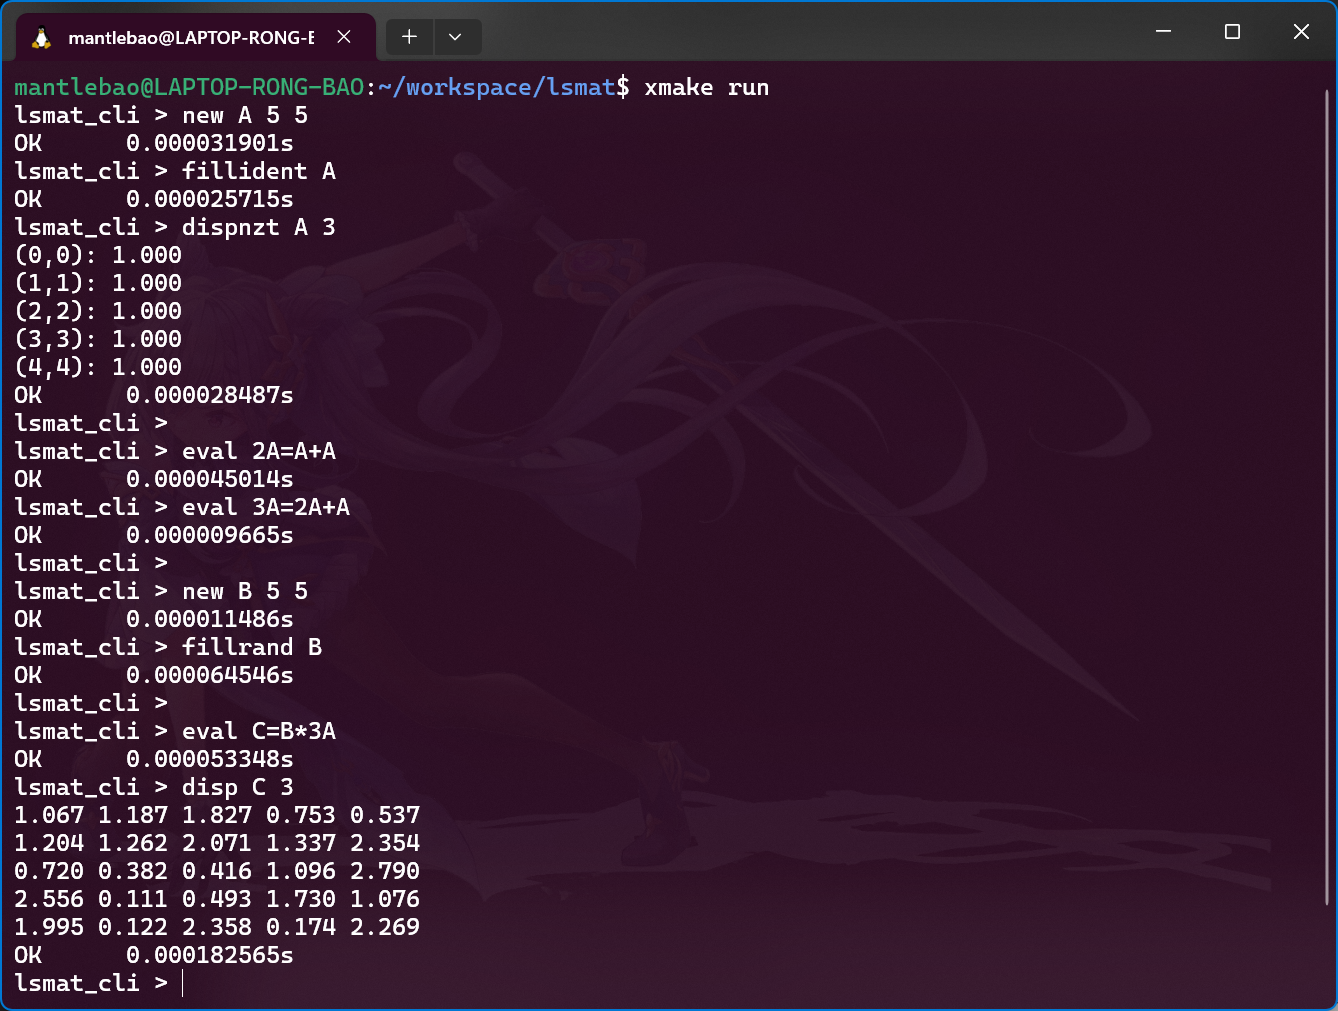
\includegraphics[scale=0.4]{cli_screenshot}
    \caption{\texttt{lsmat\_cli} 用户交互界面某一次运行的终端截图}
    \label{fig_screenshot_cli}
\end{figure}

\subsection{性能测量}

我们以运行时间和内存空间消耗量化稀疏矩阵实现的效率. 我们在上述控制台交互界面中加入计时功能, 测量用户每一条指令执行的时间消耗. 我们通过在稀疏矩阵库中的每一次内存分配时加入可选的钩子函数调用, 以统计内存分配情况.

\section{结果分析}

\begin{figure}
    \centering
    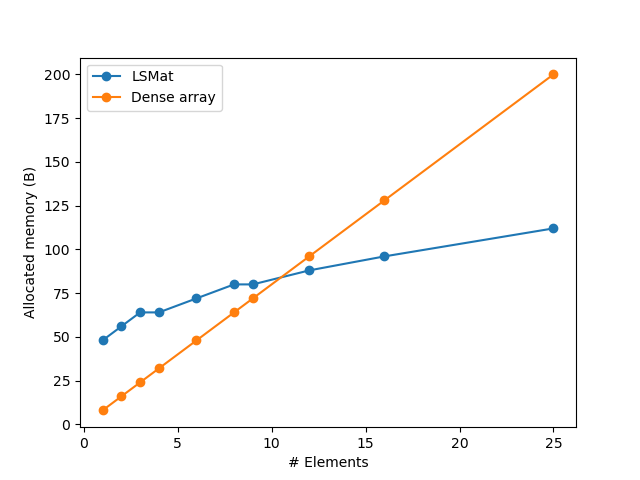
\includegraphics[scale=0.7]{lsmat_plot_mem_zero}
    \caption{稀疏矩阵与稠密数组存储全零矩阵的内存占用对比}
    \label{fig_lsmat_plot_mem_zero}
\end{figure}

\begin{figure}
    \centering
    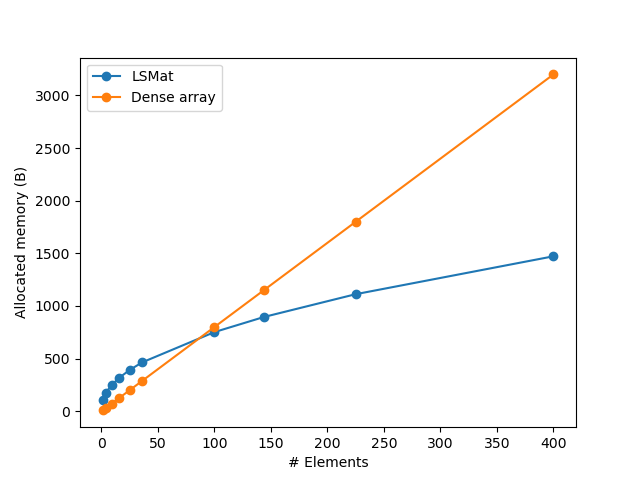
\includegraphics[scale=0.7]{lsmat_plot_mem_identity}
    \caption{稀疏矩阵与稠密数组存储单位阵的内存占用对比}
    \label{fig_lsmat_plot_mem_identity}
\end{figure}

\begin{figure}
    \centering
    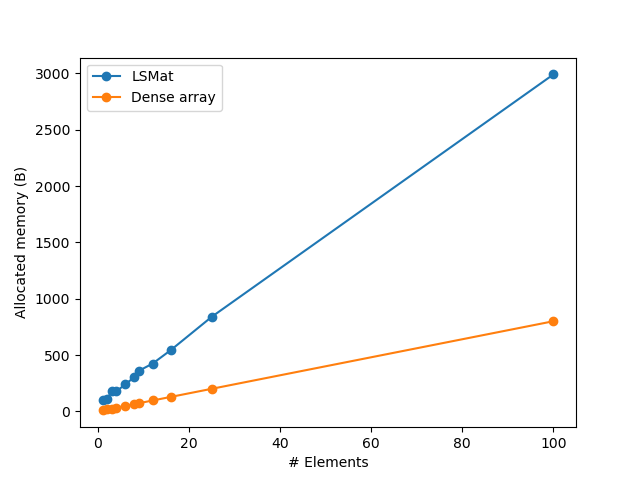
\includegraphics[scale=0.7]{lsmat_plot_mem_halfzero}
    \caption{稀疏矩阵与稠密数组存储一半元素非零矩阵阵的内存占用对比}
    \label{fig_lsmat_plot_mem_halfzero}
\end{figure}

\section{小结}

TODO.

\begin{thebibliography}{}

\bibitem{bib_numpy} Van der Walt, S.; Colbert, S. C.; Varoquaux, G. The NumPy Array: A Structure for Efficient Numerical Computation \textbf{[J]}. \textit{Computing in Science \& Engineering}, 2011, 13(2): 22-30. DOI:\href{https://doi.org/10.1109/MCSE.2011.37}{10.1109/MCSE.2011.37}.

\end{thebibliography}

\appendix

\section{附录: 算法实现}

本节给出本文实现的算法的源代码.

\subsection{稀疏矩阵基础设施}

\lstinputlisting[language=C]{./../../include/lsmat/lsmat.h}

\lstinputlisting[language=C]{./../../src/lsmat/lsmat.c}

\subsection{矩阵运算}

\lstinputlisting[language=C]{./../../include/lsmat/lsarith.h}

\lstinputlisting[language=C]{./../../src/lsmat/lsarith.c}

\subsection{用户交互界面}

\lstinputlisting[language=C]{./../../src/cli/main.c}

\section{附录: 源代码可见性}
\label{appendix_source_code}

本项目代码可于 \url{https://github.com/CSharperMantle/lsmat} 获取, 并在 BSD 3-Clause 许可证的条件与条款下使用. 授权协议的具体信息见上述 URL.

\section{附录: 课程思政报告}
\label{appendix_ideology}

TODO.
